\section{Filesystem Design}
To explore a new way of writing reliable filesystem code, using Ada, we implemented a small, prototype filesystem (AdaFS).
This section describes its design, the decisions that influenced it, and the compromises that we made.

\subsection{Design Overview}
AdaFS is based on the MINIX 2 filesystem \cite{tanenbaum1997}, with some simplifications due to time constraints.
The MINIX operating system was written by Andrew Tanenbaum as an educational tool, and is compatible with UNIX, but has a more modular structure.
We selected the MINIX filesystem as a model because it is not part of the operating system, but rather runs entirely as a user program.
As such, it is self-contained.
Furthermore, due to its educational purpose, it is thoroughly commented and easy to understand.
We chose the second version of the filesystem because MINIX 3 is more complex, as it adds numerous improvements (e.g. for reliability) to place emphasis on its use in research and production \cite{minix3history}.

\autoref{fig:design overview} shows an overview of the filesystem's design.
There are four main components: the code defining the filesystem's logic, the component responsible for disk reads and writes, the filesystem operations interface, and the FUSE driver.
When a request is sent from a userspace application (number 1 in \autoref{fig:design overview}), this request goes to the FUSE kernel module (2), which forwards it to the handler registered via the FUSE library (3).
The handler is part of the FUSE driver (4), which is currently written partially in C, and partially in Ada.
The FUSE driver calls the appropriate filesystem operation from the operations interface component (5).
This component then calls functions from the verified filesystem logic component (6), as well as the disk IO component (7), as needed.
Finally, it sends a response back up the chain of communication (from 5 back to 1).

\begin{figure}[tb]
  \centering
  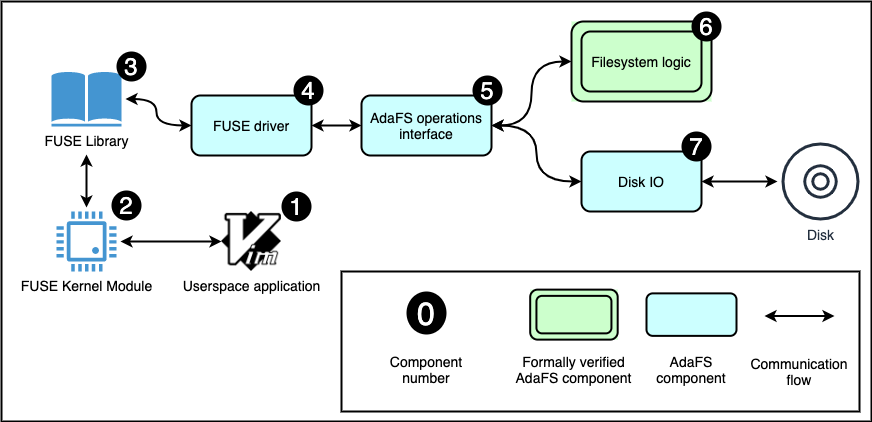
\includegraphics[scale=0.56]{design-overview.png}
  \caption{AdaFS design overview.}
  \label{fig:design overview}
\end{figure}


\subsection{Filesystem Organisation}
We next give an overview of the layout of the filesystem on disk, as well as the layout of various structures used in the filesystem.

A disk is formatted as an AdaFS filesystem using the \textit{mkfs} utility.
The resulting disk layout is shown in \autoref{fig:adafs disk layout}.
The disk is divided into blocks of 1024 bytes, similarly to MINIX.
Blocks are collected into zones, which can be of size $2^n$ blocks.
This abstraction of blocks into zones can make it possible to allocate multiple blocks at once.

\begin{figure}[tb]
  \centering
  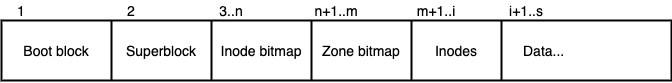
\includegraphics[scale=0.7]{disk-layout.png}
  \caption{AdaFS disk layout. (\textit{n} = number of inode bitmap blocks, \textit{m} = number of zone bitmap blocks, \textit{i} = number of inode blocks, \textit{s} = number of blocks on disk)}
  \label{fig:adafs disk layout}
\end{figure}

The disk begins with a boot block that would optionally contain executable code.
Then, it contains a superblock, and two bitmaps.
The bitmaps are used for inode and zone allocation, and can potentially span multiple blocks.
Next, there are a few blocks containing space for inodes, potentially with more than one inode per block.
Finally, the rest of the blocks contain user data.

The superblock is the second block on the disk, and contains information about the layout of the filesystem.
In particular, it contains the number of inodes and zones on disk, the number of inode and zone bitmap blocks, the number of the first data zone, the base-2 logarithm of the number of blocks per zone, the maximum file size, and the magic number.
The magic number used to identify a correctly formatted disk is $\text{CACA}_{16}$; MINIX uses the magic number $2468_{16}$, but AdaFS avoids using the same number, because a disk formatted by the AdaFS \textit{mkfs} utility is not necessarily equivalent to a disk formatted by the MINIX \textit{mkfs} utility.

The two bitmaps keep track of available inodes and zones, where the \textit{n}th bit of the inode or zone bitmap corresponds to the \textit{n}th inode or zone on disk, respectively.
If a bit in the inode bitmap is set to 1, that means the corresponding inode is allocated, and if it is set to 0, the inode is free.
This is the same for the zone bitmap, pertaining to zones.
One difference with MINIX is that, in MINIX, the first bit (bit number 0) in the bitmaps must always be allocated, as the procedure that searches for a free inode or zone returns zero if no free inode/zone is found.
In Ada, indexing generally starts at 1, so all bits can be used -- as the first bit is bit number 1, this does not interfere with the allocation procedure.

The penultimate section of the disk contains inodes; the number of inodes is determined by the size of the disk.
The inodes have two representations: on-disk (\autoref{fig:inode on disk}) and in-memory (\autoref{fig:inode in memory}).
This allows the filesystem to make efficient use of disk space, while providing faster access to important values when the inode is loaded in memory.
There are 10 zones per inode: 7 direct zones (those that contain data), 1 single indirect zone (indicates a block that contains more direct zones), 1 double indirect zone (indicates a block that contains more single indirect zones), and 1 unused zone.
The unused zone is present for future use, potentially as a triple-indirect zone.

\begin{figure}[tb]
     \centering
     \begin{subfigure}[b]{0.45\textwidth}
         \centering
         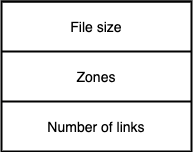
\includegraphics[scale=0.6]{inode-on-disk.png}
         \caption{On disk}
         \label{fig:inode on disk}
     \end{subfigure}
     \begin{subfigure}[b]{0.45\textwidth}
         \centering
         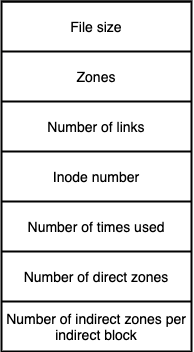
\includegraphics[scale=0.6]{inode-in-memory.png}
         \caption{In memory}
         \label{fig:inode in memory}
     \end{subfigure}
     \caption{Inode representations.}
     \label{fig:inode representations}
\end{figure}


The final section spans the rest of the blocks on the disk, broken into zones, and is available to store user data.
It can contain file data, or directory entries.

There are also some in-memory structures for working with open files.
The filesystem keeps a process table in memory, which is indexed by process ID (PID), and keeps track of inode information for all processes using the filesystem.
One entry corresponds to one process, and contains the inode numbers for the root and working directories of the process, as well as the list of open file descriptors.
Each open file descriptor corresponds to an entry in the filesystem's \textit{filp} table, which is shared among all processes and contains all of the file positions.
The rationale for a shared file position table comes from MINIX, and is based on problems with the semantics of the \textit{fork} system call \cite{tanenbaum1997}.
An entry in the filp table contains the number of file descriptors using that entry, the inode number, and the file position for the inode.

Due to time constraints, a number of simplifications were made compared to MINIX.
In particular, only the features necessary for basic functionality of the system were implemented, and only \textit{readdir} and file operations are supported (create, read, write, delete).
The filesystem does not cache any information, and there is no in-memory inode table; all data are written directly to disk.
Furthermore, the current implementation does not keep track of file mode, owner, group, or timestamps.
This results in a limited filesystem, which nonetheless completes its function as a proof-of-concept.
